\addchap{Introduction}
\label{chapter:introduction}

\todo{Make Zenodo repositories for everything relevant and add the links in the thesis. We should have at least: pytree,
peanut, cashew, ratatouille, org\_attach (?), calibration\_analysis, journal\_extract, g5k\_test (*2), hpl,
platform-calibration}


\addchap{Scientific Computing: a story}
\label{chapter:context}

    %% TODO Historique : https://fr.wikipedia.org/wiki/Superordinateur#Historique_des_records

    \addsec{First computers, from carbon to silicon}%
    \label{sec:first_computers}

        % TODO talk about the human computers, followed by the first (machine) computer created by Cray and IBM, also
        % Von Neuman, analog computers, etc.
        Science has always been tightly associated to computations, hence this is no surprise that the first computers
        were not machines, but humans. Already in the second century AD, Ptolemy, a scientist living in Alexandria,
        wrote the Almagest. This book aggregated the state of the art in mathematics and astronomy and remained a
        reference for centuries. It contained several tables that were computed by the scientist, including a
        trigonometric table (called \emph{table of chords}).

        In 1757, three French astronomers, Clairaut, Lalande and Lepaute, started working on the prediction of the next
        appearances of Halley's comet~\cite[Chapter~1]{human_computers}. Using the recent theories of Newton, they had
        to numerically solve the three-body problem: they computed the orbits of Saturn and Jupiter around the Sun,
        taking into account the attraction force between the two planets. They carried this computation by splitting the
        orbits in tiny steps, computing the new planet locations for each step. They used these sequences of coordinates
        to compute the orbit of Halley's comet around the Sun, by taking into account the effect of the two giant
        planets on the comet and neglecting the effect of the comet itself on the three bodies. They were succesful in
        predicting the next appearance of the comet in the beginning of 1759, making an error of only one month. Their
        work constitutes one of the first recorded division of labor applied to computations, Lalande and Lepaute
        computed the orbits of the two giant planets while Clairaut computed the orbit of the comet.

        Gaspard de Prony, a French civil engineer, went a step further in this endeavor of organized
        computation\cite[Chapter~2]{human_computers}. In 1791, he was named director of the \emph{Bureau du Cadastre}.
        At the time, the French revolutionary government was preparing reforms for their outdated system of weights and
        measures, which will eventually result in the creation of the metric system. The reforms proposed to measure
        angles in grades instead of degrees, dividing a right angle into 100 grades instead of 90 degrees. Prony was
        tasked to prepare trigonometric tables for this decimal grade system. He organized his staff in a hierarchy of
        three levels:
        \begin{itemize}
            \item The first class of workers, a handful of renowed scientists like Carnot or Legendre, oversaw the
                operations. They had to research the appropriate formulas for computing approximations of trigonometric
                functions with basic arithmetical operations.
            \item The second class, subsequently named \emph{planning commitee}, was a team of eight experienced
                computers. Their task consisted in translating the trigonometric equations produced by the first class
                into a sequence of additions and substractions. They prepared worksheets where all the basic operations
                were written with a blank space for the result.
            \item The third class consisted in nearly ninety computers. Many of them were former servants or wig makers
                that lost their jobs with the Revolution, they did not know any mathematics besides the addition and
                substraction. Their job was to compute the results to fill the blank spaces left by the second class of
                workers.
        \end{itemize}

        The idea of constructing a machine capable of doing computations is not recent. Already in 1642, Blaise Pascal,
        a French mathematician, invented and built a mechanical calculator that could perform the four arithmetical
        operations. The calculator was not commercialy viable at the time, so only twenty machines were built. Much
        later, in the first half of the nineteenth century, Charles Babbage~\cite[Chapters~2-3]{human_computers}, an
        English mathematician, invented two very innovative machines. The difference engine, for computing tables of
        polynomial functions, and the analytical engine, a general purpose computer that would subsequently be qualified
        as \emph{Turing-complete}. Unfortunately, due to a lack of funding, he was never able to build his inventions.
        In the same period, a French inventor named Thomas de Colmar designed and manufactured a digital
        mechanical calculator, called arithmometer. Capable of doing the four arithmetical operations, it was the first
        machine of its kind to be reliable enough for a practical use.  Similarly, Herman Hollerith, an American
        inventor, created the tabulating machine. Initialy built to process the 1890 US Census data, it worked by
        reading and summarizing information stored in punched cards. It decreased considerably the duration and cost of
        the whole census organization. These two last inventions~\cite[Chapter~6]{human_computers} were commercial
        successes and started an era of mechanical computations that lasted until the second half of the twentieth
        century.


        \todo{Add some text on the human computers at NASA, the first IBM computer.}

    \addsec{Exponential growth}%
    \label{sec:exponential_growth}

        % TODO Moore's law, huge performance gains, helped to get great scientifical breakthrough
        % Not terminated yet, we "need" to go further. Side note: when will it be enough? Question of the environmental
        % impact (we make great progress in terms of efficiency, like flops/W, but the growth is even faster (so for
        % instance the total consumptions are still increasing)).

        \begin{figure}[htbp]
            \centering
            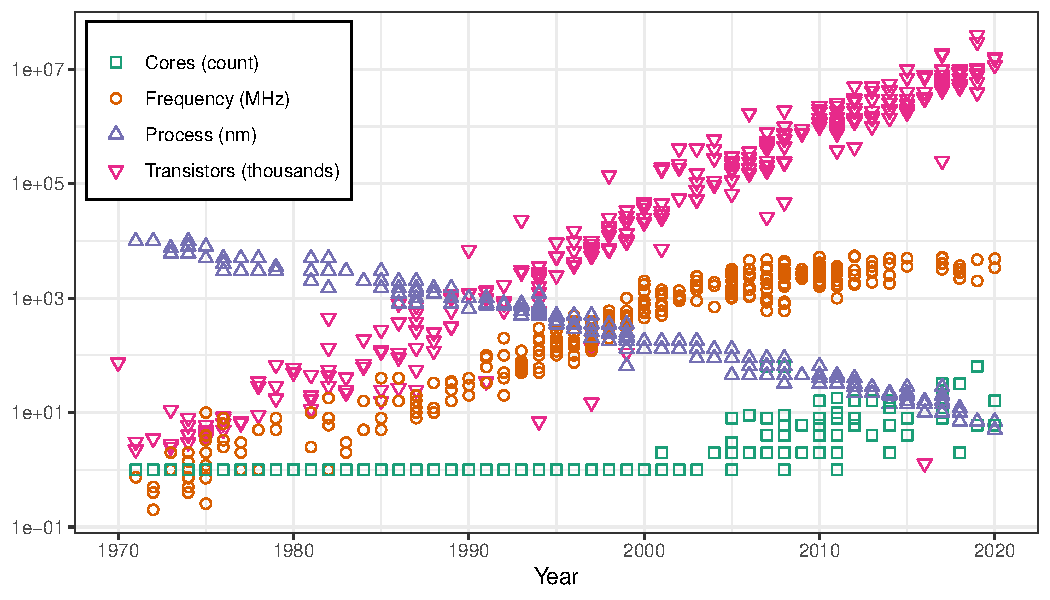
\includegraphics[width=\textwidth]{img/context/49_years.pdf}
            \caption{\label{fig:context:49_years}
            Evolution of the processor characteristics between 1971 and 2020. Plot inspired from the work of Pedro Bruel,
            generated with data from wikipedia~\cite{wiki2021chronology,wiki2021transistor}.}
        \end{figure}


        \begin{figure}[htbp]
            \centering
            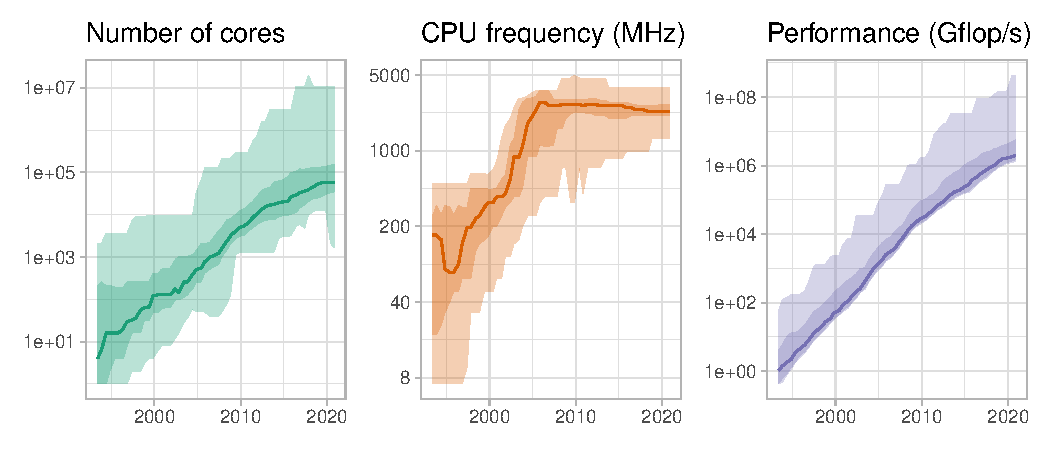
\includegraphics[width=\textwidth]{img/context/top500.pdf}
            \caption{\label{fig:context:top500}
            Evolution of the Top500~\cite{top500} supercomputers between 1993 and 2020.  The line denotes the median, the inner ribbon
            contains the \([\NSI{10}{\percent}, \NSI{90}{\percent}]\) interval, the outer ribbon contains all the
            values.\\ Data compiled by Dan Lenski~\cite{top500_compiled} and plotted by ourselves.}
        \end{figure}


    \addsec{Increased complexity}%
    \label{sec:increased_complexity}

        % TODO increased complexity everywhere (HW and SW), deterministic at micro-level but the macro-level is random
        % no complete understanding of the whole thing, we need experimental CS, we need models (very similarly to what
        % is done in physics or biology)
        Some horror stories\cite{Petrini_2003}\dots
